\documentclass[thmsb,11pt]{article}
\usepackage{amsfonts}
\usepackage{appendix}
\usepackage[pagewise,displaymath, mathlines]{lineno}
\usepackage{amssymb}
\usepackage{amsmath}
\usepackage{graphicx}
\usepackage{color}
\usepackage{refcount}
\usepackage{natbib}
\usepackage{bm}
\usepackage{hyperref}
\usepackage{epstopdf}
\setcounter{MaxMatrixCols}{10}
\newtheorem{theorem}{Theorem}
\newtheorem{acknowledgement}[theorem]{Acknowledgement}
\newtheorem{algorithm}[theorem]{Algorithm}
\newtheorem{assumption}{Assumption}
\newtheorem{axiom}{Axiom}
\newtheorem{case}[theorem]{Case}
\newtheorem{claim}[theorem]{Claim}
\newtheorem{conclusion}[theorem]{Conclusion}
\newtheorem{condition}[theorem]{Condition}
\newtheorem{conjecture}{Conjecture}
\newtheorem{corollary}{Corollary}
\newtheorem{criterion}[theorem]{Criterion}
\newtheorem{definition}{Definition}
\newtheorem{lemma}{Lemma}
\newtheorem{problem}[theorem]{Problem}
\newtheorem{proposition}{Proposition}
\newtheorem{solution}[theorem]{Solution}
\newtheorem{summary}[theorem]{Summary}
\newtheorem{example}{Example}
\newtheorem{exercise}{Exercise}
\newtheorem{notation}{Notation}
\newtheorem{remark}{Remark}
\newcommand{\bmat}{\begin{matrix}}
\newcommand{\emat}{\end{matrix}}
\newcommand{\ov}{\overline}
\newcommand{\un}{\underline}
\newcommand{\EE}{\mathbb E}
\newenvironment{proof}[1][Proof]{\noindent \textbf{#1.} }{\  \rule{0.5em}{0.5em}}
\topmargin=-1cm
\oddsidemargin=-0cm
\textheight=22.2cm
\textwidth=16cm
\setcounter{secnumdepth}{2}
\pagestyle{plain}
\setcounter{figure}{0}
%\setpagewiselinenumbers
%\linenumbers
\begin{document}

\title{\textbf{ Notes on BEGS with $N>2$ types}}
\maketitle
\section{Results}
As discussed we had 4 results governing the long run distribution of assets we wished to check with more than two types of agents: 
\begin{description}
	\item[\textbf{Spanning}:]  In the long run agents with lower productivity will hold more assets than agents with higher productivity.
	\item[\textbf{Convergence Speed}:]  That the speed of convergence depends on the correlation of the payoff of the asset with the exogenous shock.  Specifically the lower the correlation the slower the convergence.
	\item[\textbf{Imperfect Spanning}:]  With more than two states the spanning is imperfect, a sufficiently bad sequence of shocks will push you away from the steady state.
	\item[\textbf{Government Debt Level}:]  Under the normalization of the lowest productivity agent having no assets the government with a greater redistributive motive will hold less assets in the steady state.
\end{description}  We find that the first 3 conditions still hold true.  The last is more complicated with a larger number agents.

For this analysis we used the following calibration.  We set the number of agents at 10.  We assumed the agents had BGP preferences over consumption and labor given by
\[
	\psi \log(c) + (1-\psi) \log(1-l)
\]with $\psi$ set to be $0.6994$.  The discount factor was set at $0.98$ and the level of exogenous government expenditure was assumed to be constant $0.206$.  The 10 types of agents were calibrated to have productivies to roughly capture the degree of income inequality in the united states:
\[
\theta =  [  1.  ,   1.6 ,   2.45,   3.35,   4.4 ,   5.6 ,   7.  ,   8.9 ,
        12.  ,  22.  ]
\]The baseline case was a utilitarian planner placing equal weights across all agents.  Uncertainty took the form of a TFP shock which was i.i.d. with standard deviation being 3\% of TFP.
\newpage

\subsection{Spanning}  Our first condition was spanning.  In figure one we plot the asset level of each agent versus the agents productivity.  We can clearly see the inverse relationship between productivity type and asset level.
\begin{figure}[htcp]
\centering
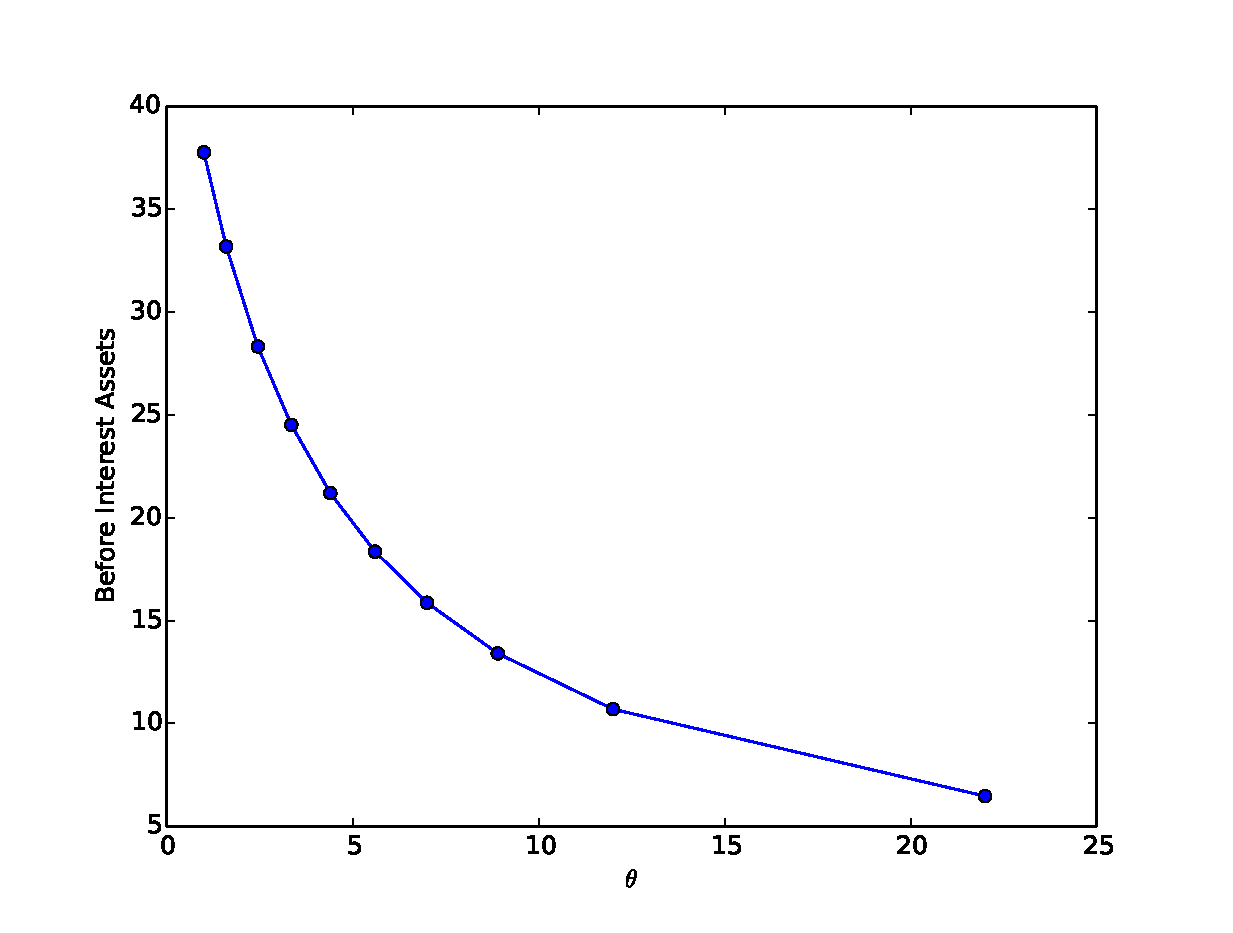
\includegraphics[width=0.7\textwidth]{Images/spanning.eps}
\caption{Assets held by agent type in steady state.}
\end{figure}
\subsection{Convergence Speed}
We next want to check how the convergence speed of the is a function of the correlation of payoffs with the exogenous shock.  Since marginal utilities are inversely proportional to TFP we changed the payoff structure of the bond from as asset which pays off uniformly in all states to an assets which pays off more in high TFP states.  Specifically the asset pays off
\[
	P_t = 1. + 0.5\epsilon_t
\]where $\epsilon$ is the TFP shock.   This reduces the correlation of the payoff, $U^i_{c,t}P_t$, with the aggregate shock.  In figure 2 we plot the time path of the ratio of marginal utilities of the lowest productivity agent to the highest productivity agent for the baseline case (blue) and the modified payoff structure case (green).  Both economies start out at the same initial distribution of Pareto weights and multipliers on the implimentability  constraint and received the same sequence of aggregate shocks.  We see that the economy with the lower correlation of payoff with aggregate shock converges to the steady state at a much slower rate.
\begin{figure}[htp]
	\centering
	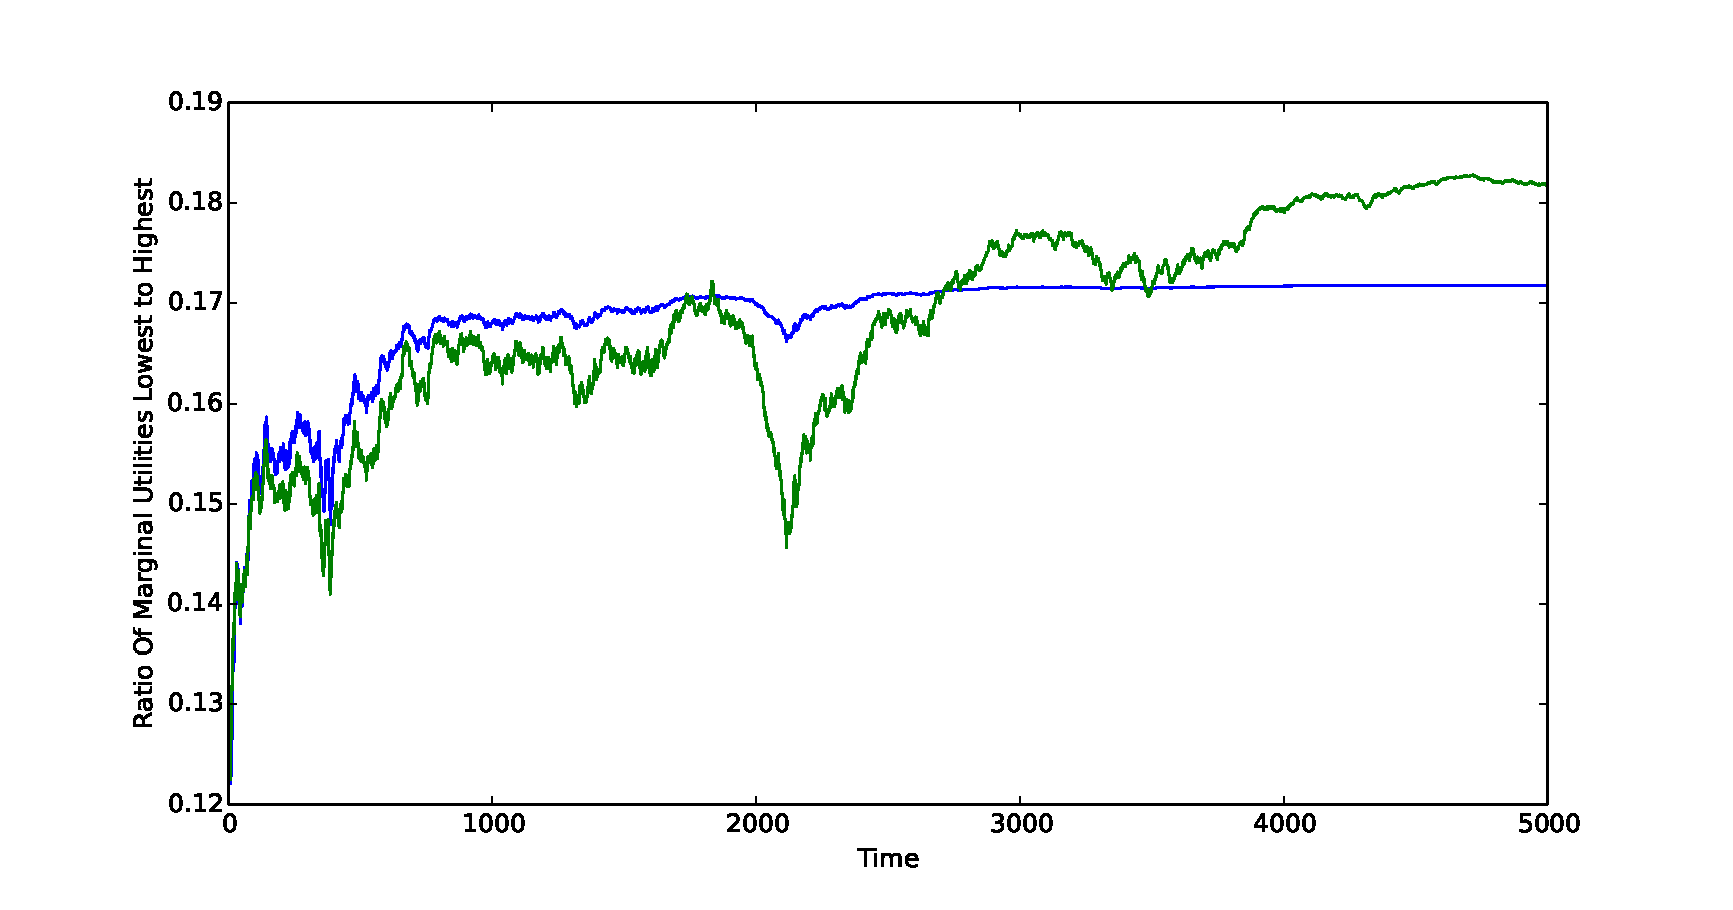
\includegraphics[width=0.7\textwidth]{Images/convergence.eps}
	\caption{Convergence of the bond economy (blue) and the modified payoff economy (green).}
\end{figure}
\newpage
\subsection{Imperfect Spanning}
To demonstrate imperfect spanning we take the steady state at the end of the long simulation of the bond economy and simulate a sequence of 120 TFP shocks which are 2 standard deviations below the mean.  In figure 3 we plot the tax rate during this sequence of bad shocks.
\begin{figure}[htp]
	\centering
	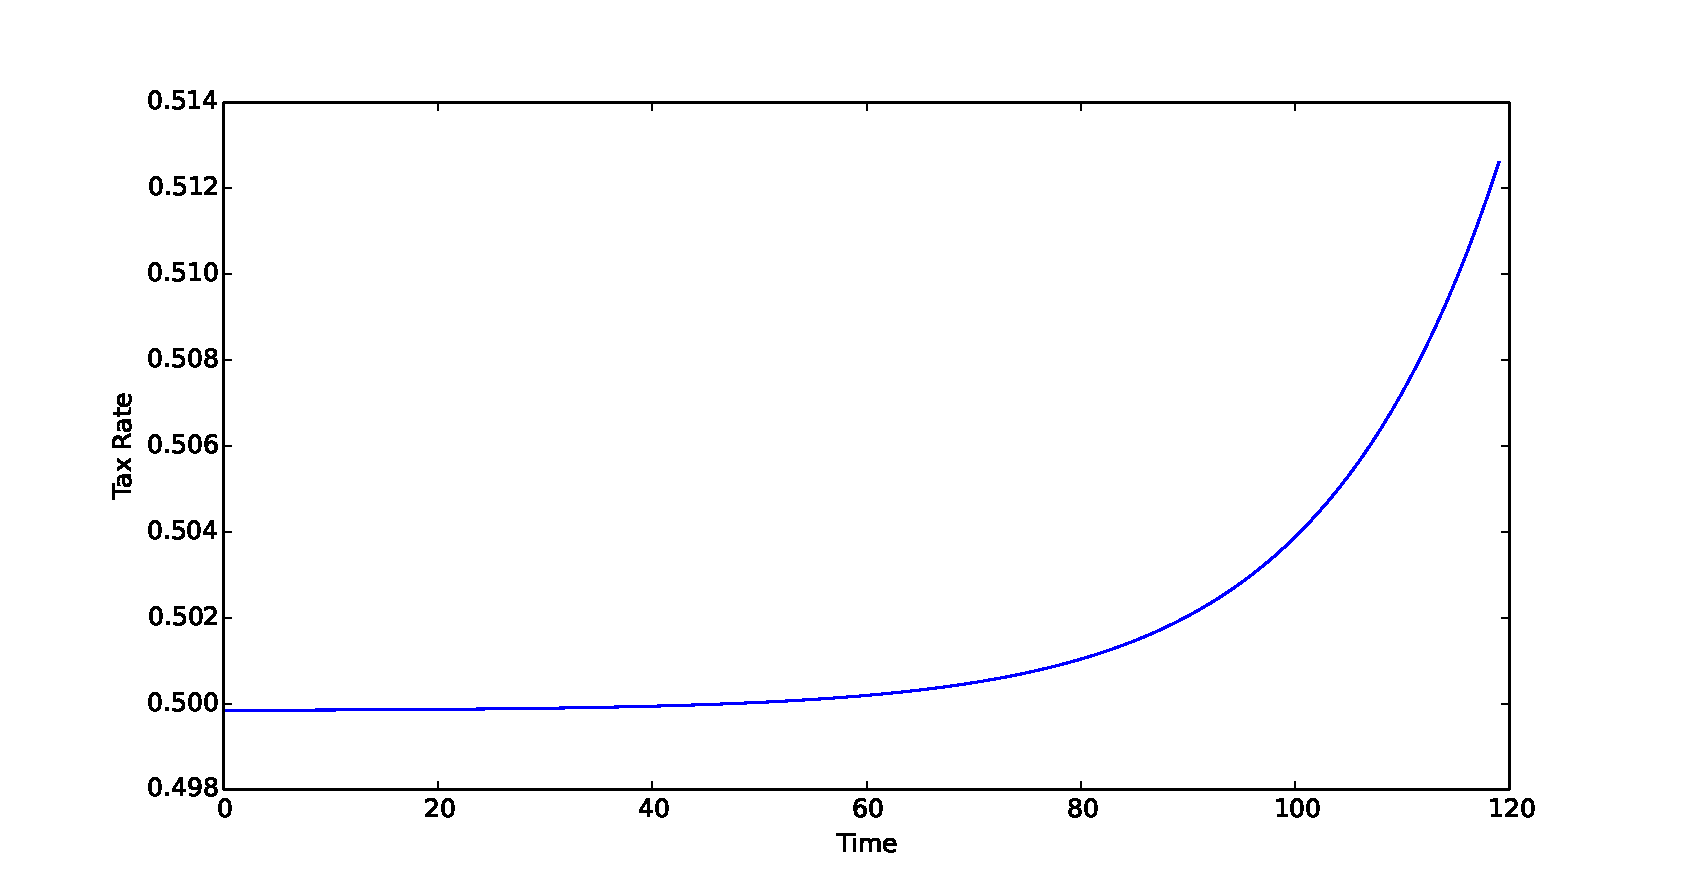
\includegraphics[width=0.7\textwidth]{Images/badshock.eps}
	\caption{Convergence of the bond economy (blue) and the modified payoff economy (green).}
\end{figure}  We see that given a sufficiently long enough sequence of bad shocks the economy will eventually deviate significantly from its steady state level.
\newpage
\subsection{Government Debt Level}  Our final conclusion was that the assets held by the government in the steady state was decreasing in the redistributive motive of the government.  This is under the normalization that the agent with the lowest productivity holds zero assets.  We check this last part by changing the Pareto weights of the government.  In our baseline case the government places equal Pareto weights on all agents.  We introduce a redistributive motive through a parameter $\alpha$.  The planner places evenly spaced Pareto weights from $0.1-\alpha$ on the lowest productivity agent to $0.1+\alpha$ on the highest productivity agent.  For example when $\alpha = 0.025$ the vector of Pareto weights will be
\[
[ 0.075     ,  0.081  0.086,  0.092,  0.097,
        0.103  0.108  0.114,  0.119 , 0.125     ]
\]As alpha increases the redistributive motive decreases.  We plot total assets of the government in steady state as a function of alpha in figure 4 and see that the relationship does indeed hold.
\begin{figure}[htp]
	\centering
	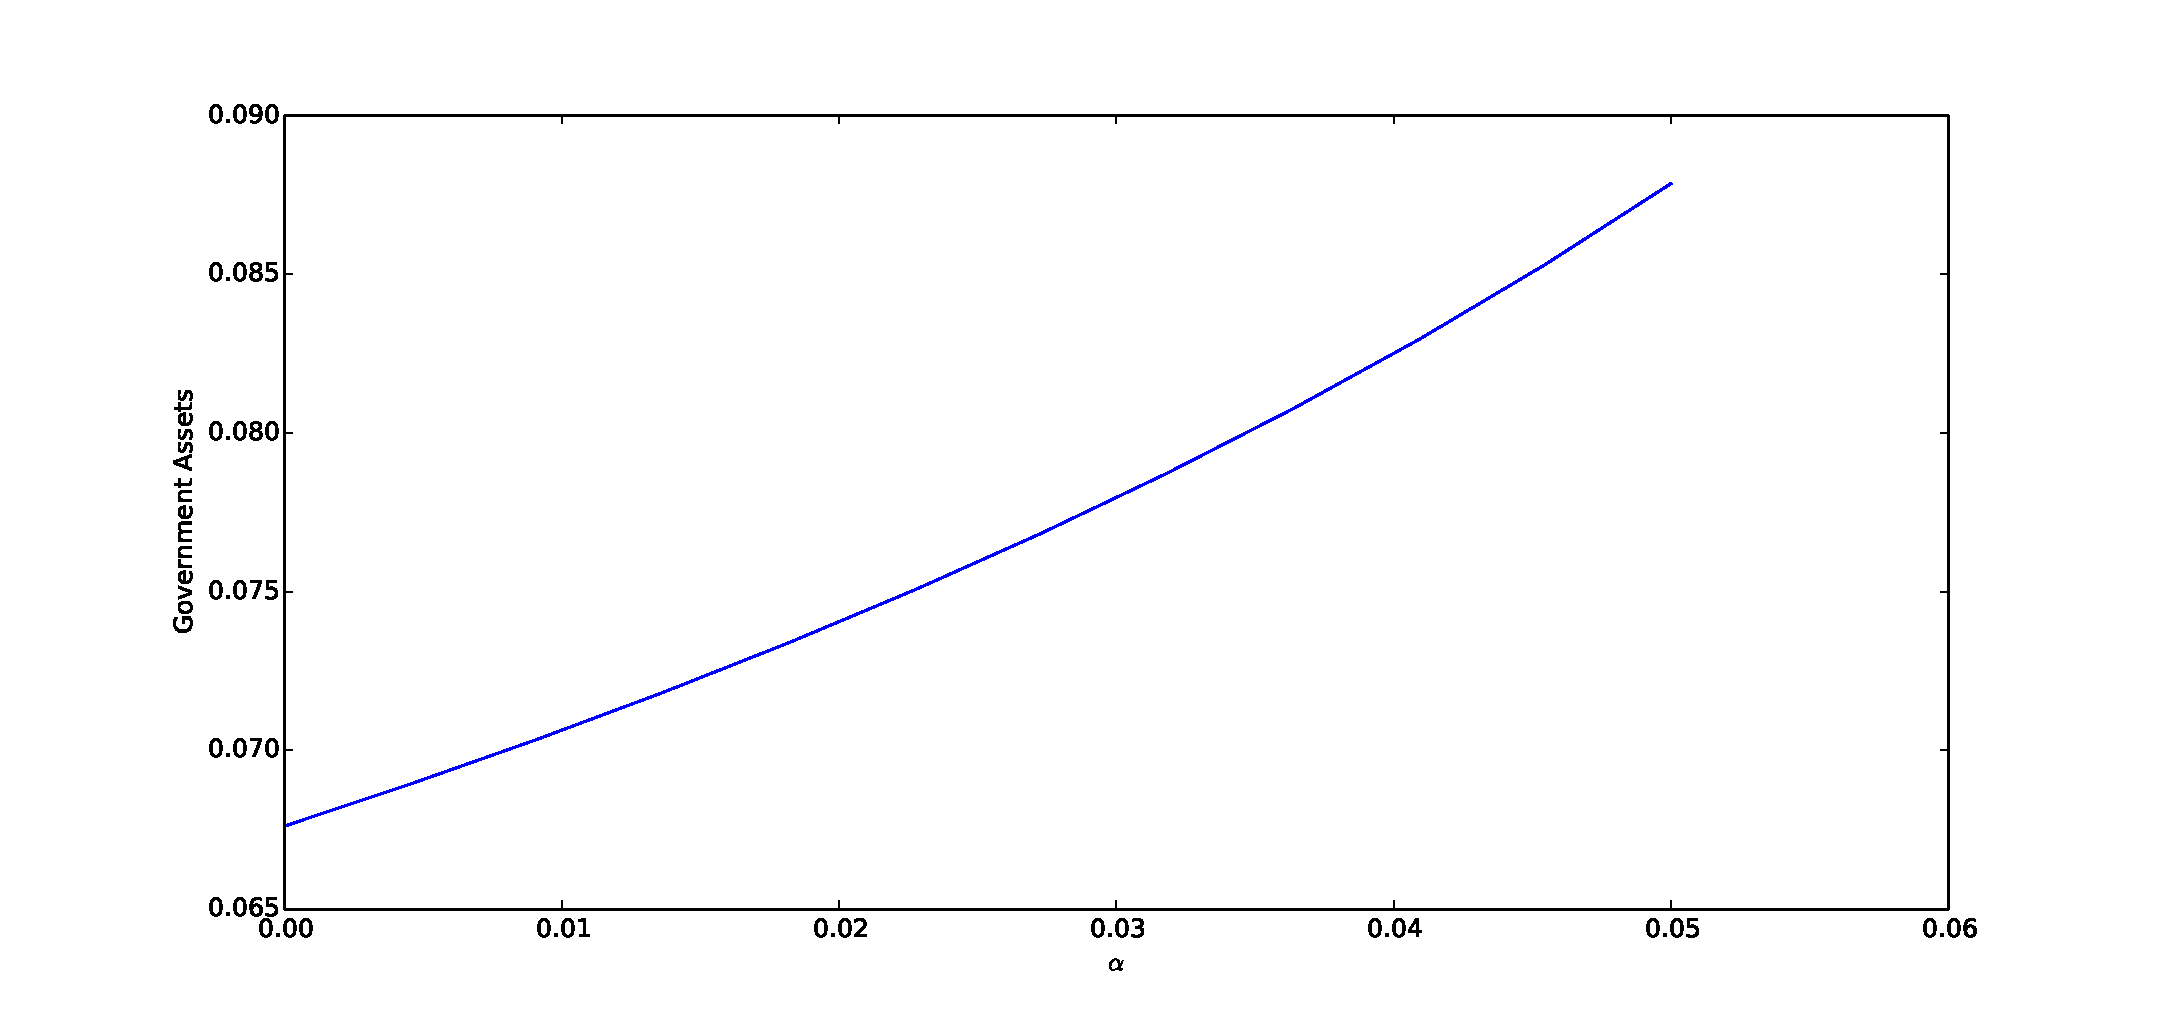
\includegraphics[width=0.69\textwidth]{Images/comp_statics.eps}
	\caption{Steady state level of government assets as a function of $\alpha$ (governing redistributive motive)}
\end{figure}

\end{document}